% Includable chapter; uses amsmath, amssymb, algorithm, algpseudocode,
% tikz, hyperref, caption. These are already present in the main notes.
\chapter{Changing state, preserving truth:  the Imperative model of computation}
\label{chap:imperative}
\vspace{-0.5in}
%\noindent{\LARGE\itshape The Imperative model of computation}\par\bigskip
\begin{center}
\begin{minipage}[t]{0.48\textwidth}
\centering\vspace{0pt}
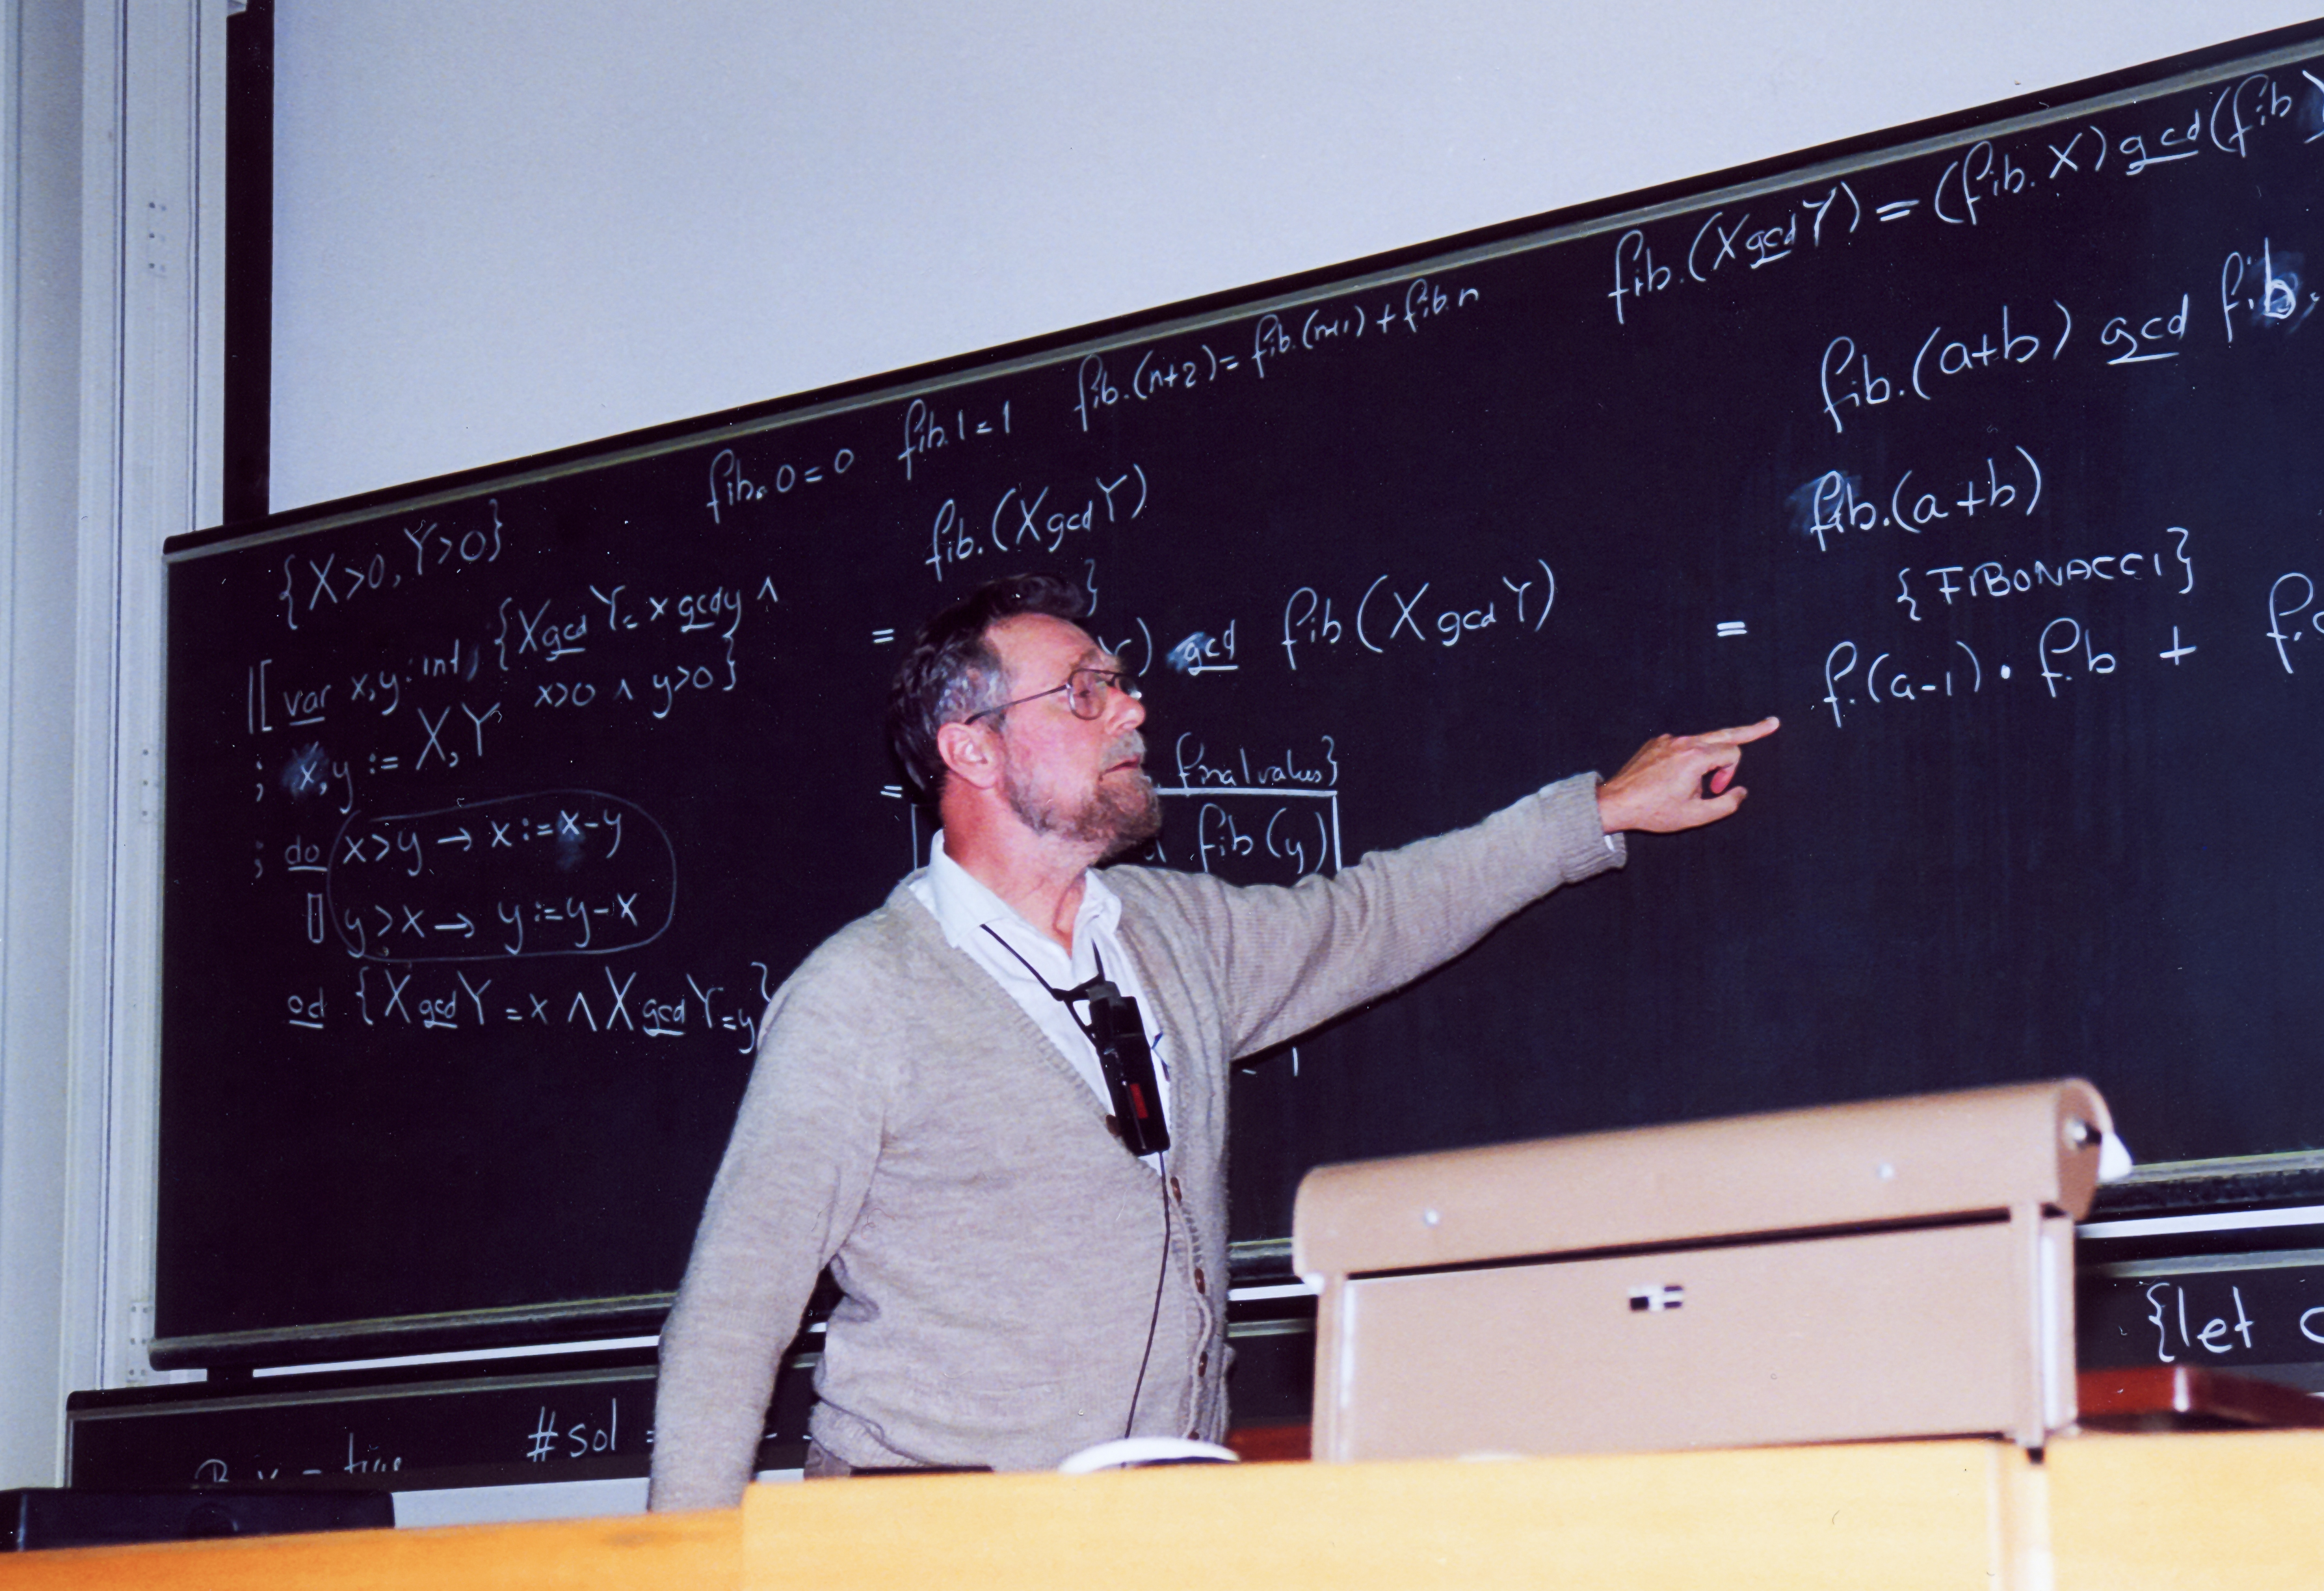
\includegraphics[height=1.12in]{images/dijkstra-1994.jpg}
\captionof*{figure}{\small ``one designs the correctness proof and derives
the program from that proof.''\\
---Edsger W. Dijkstra, \href{https://www.cs.utexas.edu/~EWD/transcriptions/EWD10xx/EWD1073.html}{EWD~1073} (excerpt).}
{\scriptsize ETH Zurich, 1994. Photo: Andreas F. Borchert,
\href{https://creativecommons.org/licenses/by-sa/4.0/}{CC BY-SA 4.0}.}
\end{minipage}\hfill
\begin{minipage}[t]{0.48\textwidth}
\centering\vspace{0pt}
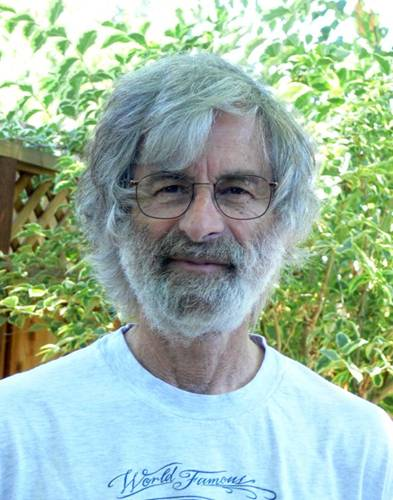
\includegraphics[height=1.12in]{images/lamport.jpg}
\captionof*{figure}{\small ``Invariants play an important role in understanding
algorithms and programs.''\\
---Leslie Lamport, \href{https://lamport.azurewebsites.net/pubs/state-machine.pdf}{\emph{Computation and State Machines}}, Section~5.1.1.}
{\scriptsize \href{https://awards.acm.org/award_winners/_1205376.cfm}{2013 Turing Award}. Photo courtesy Leslie Lamport.}
\end{minipage}
\end{center}

In Chapter~\ref{chap:algorithms}, an iterative computation passed its current state
to the next call. For factorial, the state $(k,p)$ was replaced by
$(k-1,pk)$ until $k=0$. The invariant $p\cdot k!=n!$ explained why the
answer survived each change. We now describe the same process by storing
$k$ and $p$ and giving instructions that change their contents.

This is the \emph{imperative model}: a computation is a sequence of
commands that transform a stored state. We will keep asking two questions.
What changes when a command is performed? What remains true despite that
change? The first describes the computation; the second helps us design it
and prove that it works.

Our procedures use mathematical notation and ordinary instructions, in the
style of the ruler-and-compass constructions. They do not depend on a
particular programming language. The available actions will be stated in
each setting: storing a number, exchanging two entries, placing a tile, or
moving a disk. A more detailed implementation would explain how to carry
out these actions on a particular machine.

\section{Variables become places to store values}

In the equation $y=x+1$, the letters denote mathematical values. In a
functional call $F(4,1)$, the parameters receive those values for that call;
a later call $F(3,4)$ has a new set of parameter values. Neither changes
the meaning of the earlier call.

An imperative variable has a different role. Think of it as the name of a
storage location, or a labelled box. The name stays the same while the
value in the box may change. A \emph{state} is a snapshot of the contents
of the boxes. To describe the complete progress of a computation we also
need to know which instruction comes next.

We write $x\leftarrow e$ for \emph{assignment}: evaluate the expression
$e$ using the current contents of the variables, and then store the result
in $x$, replacing its previous contents. Other locations retain their
contents. Thus $x\leftarrow x+1$ is a perfectly sensible command. If $x$
contains $4$, it will contain $5$ afterwards. The equation $x=x+1$, by
contrast, is false for every integer $x$. We reserve $=$ for equality.

\begin{figure}[ht]
\centering
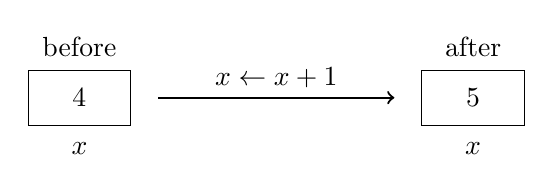
\begin{tikzpicture}
\node at (0,0.65) {before}; \node at (5,0.65) {after};
\draw (-0.65,-0.35) rectangle (0.65,0.35);\node at (0,0) {$4$};\node at (0,-0.65) {$x$};
\draw (4.35,-0.35) rectangle (5.65,0.35);\node at (5,0) {$5$};\node at (5,-0.65) {$x$};
\draw[->,thick] (1,0)--(4,0) node[midway,above] {$x\leftarrow x+1$};
\end{tikzpicture}
\caption{The location retains its name; assignment replaces its contents.}
\end{figure}

Start with $x=4$ and perform $y\leftarrow x$ followed by $x\leftarrow x+1$.
The final state is $x=5$, $y=4$. The first command copied a value; it did
not make $y$ follow all later changes to $x$. In our model, differently
named scalar variables denote separate locations. Every variable must be
assigned a value before an instruction reads it.\footnote{Real languages
also offer ways for several names to refer to the same storage. We do not
need that additional complication here. Our mathematical integers have no
fixed upper limit; a machine implementation must provide suitable storage.}

In the procedure displays, comments beginning with \texttt{\# PRE},
\texttt{\# INV}, and \texttt{\# POST} state the required initial condition,
loop invariant, and promised final condition. A \texttt{\# BOUND} comment
states a decreasing bound function for termination, defined below. A \texttt{\# ASSERT} comment
records an intermediate fact. They are mathematical statements, not
instructions. A straight-line procedure has intermediate assertions rather
than a loop invariant.

\subsection{Order matters: exchanging two values}

Suppose $x$ and $y$ initially contain $A$ and $B$. Here $A$ and $B$ are
fixed mathematical names for the original values, not locations that the
procedure changes. We want to finish with $x=B$ and $y=A$.
The commands $x\leftarrow y$ followed by $y\leftarrow x$ do not achieve
this: the first destroys the old value of $x$, and both boxes finish with
$B$. We must save the value before overwriting it.

\begin{algorithm}[H]
\begin{algorithmic}[1]
\Procedure{Exchange}{$x,y$}
\Statex \texttt{\# PRE:} $x=A$, $y=B$; $A,B$ are fixed original values.
\State Store the current contents of $x$ in a temporary location $t$.
\Statex \texttt{\# ASSERT:} $t=A$, $x=A$, $y=B$.
\State $x\leftarrow y$
\Statex \texttt{\# ASSERT:} $t=A$, $x=B$, $y=B$.
\State $y\leftarrow t$
\Statex \texttt{\# POST:} $x=B$, $y=A$.
\EndProcedure
\end{algorithmic}
\caption{Exchange the contents of two specified locations.}
\end{algorithm}

\[
\begin{array}{c|ccc}
 &x&y&t\\\hline
\text{initially}&A&B&\text{unused}\\
\text{after the first command}&A&B&A\\
\text{after the second command}&B&B&A\\
\text{after the third command}&B&A&A
\end{array}
\]
A command reads the state left by the preceding command. Translating a
simultaneous state transition into separate assignments therefore requires
care: save any old value that will still be needed.

\section{Commands, decisions, and repetition}

We use three ways to organise commands.
\begin{enumerate}
\item \emph{Sequence}: perform commands in the stated order.
\item \emph{Selection}: \textbf{if} a condition is true, perform one block
of commands; \textbf{otherwise}, perform the other. Only the chosen block
is performed.
\item \emph{Repetition}: \textbf{while} a condition is true, perform a
block of commands, then test the condition again.
\end{enumerate}
The condition of a while loop is checked \emph{before} each repetition,
so the block may be performed zero times. Indentation identifies the
commands belonging to a block. A call to a named procedure performs its
commands and then resumes the calling procedure.

For example, to store the larger of $a$ and $b$ in $m$, use
\begin{algorithmic}[1]
\Statex \texttt{\# PRE:} $a=A$, $b=B$ are comparable values.
\If{$a\geq b$}
\State $m\leftarrow a$
\Else
\State $m\leftarrow b$
\EndIf
\Statex \texttt{\# POST:} $m=\max(A,B)$, $a=A$, $b=B$.
\end{algorithmic}
The test asks a question about the current state; it does not change either
value. An assignment changes the state. Keeping these roles separate is
essential.

\subsection{What a procedure promises}

Before designing a procedure, state its \emph{precondition}: what must be
true when it begins. State its \emph{postcondition}: what it must make
true when it finishes. For Exchange these are, respectively,
\[
x=A\ \text{and}\ y=B,\qquad x=B\ \text{and}\ y=A.
\]
An \emph{assertion} is a mathematical statement about a state at a specified
point in a procedure. It describes what we claim, rather than instructing
the machine to make the claim true. Our proof must justify it.

Correctness has two parts: the procedure must finish, and its final state
must satisfy the postcondition whenever its initial state satisfies the
precondition. A rule that would give the right answer \emph{if} it finished
is not enough to solve the problem on every permitted input.

\section{A loop invariant is an induction hypothesis}

The tail-recursive factorial construction in Section~\ref{sec:alg-iteration}, with its invariant proved in Section~\ref{sec:alg-invariants}, gives the transition
$(k,p)\mapsto(k-1,pk)$. We now store the two components and update them
with assignments. The same invariant guides these updates.

Start with the desired loop postcondition: $k=0$ and $p=n!$.
To generalise it, allow unfinished work, represented by $k!$, so that
$p\cdot k!=n!$. At $k=0$ this reduces to the required answer.
At each test of the loop condition, we therefore claim
\[
I:\qquad 0\leq k\leq n\quad\text{and}\quad p\cdot k!=n!.
\]
This is a \emph{loop invariant}. Its truth is preserved from one test of
the condition to the next, even though the values in it change.
It need not hold between every pair of commands inside the loop.


To obtain $p=n!$ at the end, let $k!$ represent the work still to do.
The invariant suggests starting with $k=n$ and $p=1$, and stopping at
$k=0$. When $k>0$, decreasing $k$ by one must be balanced by multiplying
$p$ by the old $k$, because $(pk)(k-1)!=pk!$. Thus the multiplication must
precede the decrement. We obtain the following commands from that reasoning.

\begin{algorithm}[H]
\begin{algorithmic}[1]
\Procedure{Factorial}{$n$}
\Statex \texttt{\# PRE:} $n\in\mathbb N$ is fixed.
\State $k\leftarrow n$
\State $p\leftarrow1$
\Statex \texttt{\# INV:} $k,p\in\mathbb N$, $0\leq k\leq n$, $p\cdot k!=n!$.
\Statex \texttt{\# BOUND:} $k$.
\While{$k>0$}
\State $p\leftarrow p\cdot k$
\State $k\leftarrow k-1$
\EndWhile
\Statex \texttt{\# POST:} $k=0$ and $p=n!$; $n$ is unchanged.
\State \Return $p$
\EndProcedure
\end{algorithmic}
\caption{Factorial by successive changes of state.}
\end{algorithm}

\paragraph{Initialisation.}
Before the first test, $k=n$ and $p=1$, so $I$ holds.

\paragraph{Preservation.}
Suppose $I$ holds at a test for which $k>0$. Call the values at that point
$K$ and $P$. The two commands produce $p=PK$ and $k=K-1$. Since $K\geq1$,
\[
p\cdot k!=(PK)(K-1)!=P K!=n!.
\]
The bounds on $k$ persist too. This proves preservation for one execution
of the \emph{whole} loop body.

\paragraph{Exit.}
When the condition becomes false, $k\leq0$. Together with the invariant
this gives $k=0$, and hence $p=n!$.

\paragraph{Termination.}
A \emph{bound function} assigns a nonnegative integer to each state
at a loop test. Whenever the body executes, its value must strictly
decrease from one test to the next. It therefore decreases monotonically
along the computation, and cannot decrease forever. If its initial value
is $B$, there can be at most $B$ repetitions, provided each execution of
the body itself finishes. The bound need not decrease by exactly one,
and the loop may stop before it reaches zero.

For factorial the bound function is $k$: it starts at $n$ and decreases
by one on every repetition. A bound function is also called a
\emph{loop variant}. An invariant tells us what remains true; a bound
function establishes progress towards termination. Merely never increasing
is insufficient: a constant value would permit endless repetition.
Nor is strict decrease among nonnegative real numbers enough: the sequence
$1,1/2,1/4,\ldots$ never ends. Here we use nonnegative integers.

Where was induction used? We induct on the number $j$ of completed
repetitions. The invariant holds for $j=0$. For every integer $j\geq0$,
if it holds after $j$ repetitions and another repetition is performed,
preservation shows that it holds after $j+1$. Thus it holds at every
reached test, including the final one. This is the induction principle
applied to a computation's history.

For $n=4$, the states $(k,p)$ at successive tests are
\[
(4,1),\ (3,4),\ (2,12),\ (1,24),\ (0,24).
\]
They are the same states as in the tail-recursive version. The model of
description has changed; the invariant and the computation have not.

\subsection{From the postcondition to the invariant and the loop}

We first stated the factorial postcondition, then generalised it to an
invariant before writing commands. The invariant supplied
the initial state, the update, and the stopping condition. Reversing the
two assignments would multiply by the new $k$ and break that reasoning.
This order of development applies to the remaining examples too.
Begin with the final assertion, and generalise it to describe partial
progress: replace a completed range by a growing prefix, allow an
unfinished remainder, or retain a smaller equivalent problem. Keep the
conditions that protect data and preserve the meaning of the answer.
The invariant must be weak enough to hold initially and strong enough to
yield the postcondition at exit. This is a design method, not a mechanical
recipe for finding an invariant.
For a loop with invariant $I$ and condition $C$, prove:
\begin{enumerate}
\item The initialisation establishes $I$.
\item If $I$ and $C$ hold, the body re-establishes $I$.
\item $I$ together with the failure of $C$ implies the required answer.
\item A nonnegative integer bound function strictly decreases on every
execution of the body, and each execution finishes.
\end{enumerate}
The first three establish the answer on exit; the fourth establishes that
exit is reached. A loop that repeatedly leaves $k$ unchanged can preserve
$k\geq0$ forever. Preservation alone does not imply progress.

\section{Familiar computations, now with stored state}

\subsection{Summation: the processed part and the remaining part}

Recall the recursive sum in Section~\ref{sec:alg-sum} and its iterative
form in Section~\ref{sec:alg-sum-iteration}. We now implement that same
accumulation by assignments.

Let $f:\mathbb N\to\mathbb N$ be a function whose values can always be computed, and let $a,b\in\mathbb N$.
The loop postcondition is $k>b$ and $s=\sum_{i=a}^{b}f(i)$,
taking an empty sum to be zero. Generalise the completed upper endpoint
$b$ to $k-1$: only the terms before the moving index $k$ have been added.
The inputs and the rule for $f$ remain fixed throughout the procedure.
Choose a location $s$ for the sum so far and a location $k$ for the next
index to be processed. The invariant, including the empty-interval case, is
\[
a\leq k\leq\max(a,b+1),\qquad s=\sum_{i=a}^{k-1}f(i).
\]
The empty processed part suggests $k=a$, $s=0$. To extend it by one term,
add $f(k)$ before advancing $k$.

The same invariant can be written as
\[
s+\sum_{i=k}^{b}f(i)=\sum_{i=a}^{b}f(i).
\]
Work already done and work still to do together make the whole task.
This is a useful pattern for discovering invariants.

\begin{algorithm}[H]
\begin{algorithmic}[1]
\Procedure{Sum}{$f,a,b$}
\Statex \texttt{\# PRE:} $a,b\in\mathbb N$; $f:\mathbb N\to\mathbb N$ is computable; inputs fixed.
\State $s\leftarrow0$
\State $k\leftarrow a$
\Statex \texttt{\# INV:} $s\in\mathbb N$, $a\leq k\leq\max(a,b+1)$,
\Statex \texttt{\#} $s=\sum_{t=a}^{k-1}f(t)$; $f,a,b$ unchanged.
\Statex \texttt{\# BOUND:} $\max(0,b-k+1)$.
\While{$k\leq b$}
\State $s\leftarrow s+f(k)$
\State $k\leftarrow k+1$
\EndWhile
\Statex \texttt{\# POST:} $k>b$, $s=\sum_{t=a}^{b}f(t)$ (zero for an empty interval).
\State \Return $s$
\EndProcedure
\end{algorithmic}
\caption{Accumulate the sum of successive function values.}
\end{algorithm}

Initially the sum in the invariant is empty. If the old index is $K\leq b$,
then the updated values satisfy
\[
s_{\rm new}=\sum_{i=a}^{K-1}f(i)+f(K)=\sum_{i=a}^{K}f(i),
\qquad k_{\rm new}=K+1.
\]
Thus the invariant is preserved. Induction on the number of completed
repetitions, beginning at zero and with the step valid for every integer
$j\geq0$ for which the loop continues, proves it at every test. At exit, if $a\leq b$, then $k=b+1$, so the sum is the desired one.
The bound function $\max(0,b-k+1)$ decreases by one whenever the body
executes. Each evaluation of $f$ finishes by the precondition. If $a>b$,
the loop is skipped and returns zero, as required.

The procedure evaluates $f$ exactly $b-a+1$ times when $a\leq b$.
Its total time must also include the cost of those evaluations.

\subsection{Quotient and remainder together}

Section~\ref{sec:alg-division} constructed quotient and remainder by
repeated subtraction. Here we compute both together, retaining the same
relationship that justified the inductive step. For fixed $a\geq0$ and
$b>0$, the postcondition is $a=bq+r$, $q\geq0$, and $0\leq r<b$.
Generalise it by dropping the final restriction $r<b$: the remainder may
still contain whole copies of $b$. Maintain
\[
a=bq+r,\qquad q\geq0,\quad r\geq0.
\]
Here $q$ counts the copies of $b$ already removed, while $r$ is what remains.
The invariant suggests $q=0,r=a$ initially. If $r\geq b$, subtracting
$b$ from $r$ must be balanced by adding one to $q$. Stopping when $r<b$
then gives both the quotient and the required remainder bound. These
choices follow from the relationship we have decided to preserve.

\begin{algorithm}[H]
\begin{algorithmic}[1]
\Procedure{Divide}{$a,b$}
\Statex \texttt{\# PRE:} $a,b\in\mathbb N$ and $b>0$.
\State $q\leftarrow0$
\State $r\leftarrow a$
\Statex \texttt{\# INV:} $q,r\in\mathbb N$, $a=bq+r$; $a,b$ fixed.
\Statex \texttt{\# BOUND:} $r$.
\While{$r\geq b$}
\State $r\leftarrow r-b$
\State $q\leftarrow q+1$
\EndWhile
\Statex \texttt{\# POST:} $a=bq+r$, $q\geq0$, $0\leq r<b$; inputs unchanged.
\State \Return $(q,r)$
\EndProcedure
\end{algorithmic}
\caption{Each repetition removes one more copy of the divisor.}
\end{algorithm}

Initialisation is immediate. If $a=bQ+R$ and $R\geq b$, then
$a=b(Q+1)+(R-b)$, so the full body preserves the invariant and nonnegativity.
This is induction on the number of completed subtractions, which is the
quotient counter $q$: the base is $q=0$, and the step applies to every
integer $q\geq0$ for which another subtraction is made.
At exit $0\leq r<b$, giving precisely the quotient and remainder conditions.
The bound function is the nonnegative remainder $r$; it strictly decreases on every repetition.
For $(a,b)=(17,5)$, the states $(q,r)$ at tests are
$(0,17),(1,12),(2,7),(3,2)$.

\subsection{Euclid: preserving the answer while changing the problem}

Section~\ref{sec:alg-euclid} proved the common-divisor property, and
Section~\ref{sec:alg-iterative-examples} expressed it as an invariant.
The functional transition $(u,v)\mapsto(v,\operatorname{mod}(u,v))$
preserves the gcd. To realise it with assignments, compute the remainder
before overwriting $u$.

For fixed inputs $a,b\in\mathbb N$ not both zero, the loop postcondition
is $v=0$ and $u=\gcd(a,b)$. Since $\gcd(u,0)=u$ for $u>0$,
rewrite the answer as $\gcd(u,v)=\gcd(a,b)$ at $v=0$.
Generalise by allowing $v$ to be nonzero, while keeping the gcd fixed.
This gives the invariant
\[
u,v\in\mathbb N,\qquad u+v>0,\qquad \gcd(u,v)=\gcd(a,b).
\]
Initialising $(u,v)=(a,b)$ establishes it. The common-divisor property
suggests the update above, while the stopping condition $v=0$ makes the
invariant yield $u=\gcd(a,b)$. Temporary storage lets us implement that
update without losing an old value that is still needed.

\begin{algorithm}[H]
\begin{algorithmic}[1]
\Procedure{Euclid}{$a,b$}
\Statex \texttt{\# PRE:} $a,b\in\mathbb N$, not both zero.
\State $u\leftarrow a$
\State $v\leftarrow b$
\Statex \texttt{\# INV:} $u,v\in\mathbb N$, $u+v>0$, $\gcd(u,v)=\gcd(a,b)$; $a,b$ fixed.
\Statex \texttt{\# BOUND:} $v$.
\While{$v>0$}
\State $r\leftarrow\operatorname{mod}(u,v)$
\State $u\leftarrow v$
\State $v\leftarrow r$
\EndWhile
\Statex \texttt{\# POST:} $v=0$, $u=\gcd(a,b)$; inputs unchanged.
\State \Return $u$
\EndProcedure
\end{algorithmic}
\caption{Preserve the gcd, using temporary storage for the remainder.}
\end{algorithm}

The chosen invariant holds initially. The common-divisor argument from
Section~\ref{sec:alg-euclid} proves preservation for the complete body. Induction
on the number of completed repetitions proves it at every test, with base
zero and the preservation step for every reached iteration.
On exit $v=0$, so $u=\gcd(a,b)$. The new $v$ is smaller than the old
positive $v$. Thus $v$ is a bound function, proving termination. The logarithmic bound on the
number of remainder steps from Section~\ref{sec:alg-euclid} is unchanged
by this translation.

\section{Lists and a non-numerical invariant}

Suppose a list occupies indexed locations $L[1],\ldots,L[m]$. An entry
may contain a letter, a name, or another finite object. Reading $L[i]$
retrieves that entry; assigning to $L[i]$ replaces it. We can reverse the
list by exchanging its outermost entries and moving inwards.

Let $L_0$ be the fixed original list of length $m$. Write $L[a..b]$
for an indexed segment, empty if $a>b$, and write $\operatorname{rev}(S)$
for a sequence $S$ read backwards. These describe mathematical sequences;
no extra copies need be stored. Relax the final requirement
$L=\operatorname{rev}(L_0)$ by marking exactly which segments are finished.
At each loop test the invariant is
\[
\begin{gathered}
|L|=m,\quad 1\leq\ell\leq m+1,\quad 0\leq r\leq m,\\
\ell\leq r+1,\qquad \ell+r=m+1,\\
L[1..\ell-1]=\operatorname{rev}(L_0[r+1..m]),\\
L[\ell..r]=L_0[\ell..r],\\
L[r+1..m]=\operatorname{rev}(L_0[1..\ell-1]).
\end{gathered}
\]
Thus the current left end is the reversal of the corresponding original
right end; the current right end is the reversal of the original left end;
and the entire middle is still unchanged. The two finished ends are not
asserted to be reversals of \emph{each other}. Their relation is to the
original list, which need not be a palindrome.
\[
\underbrace{L[1..\ell-1]}_{\text{finished left end}}\quad
\underbrace{L[\ell..r]}_{\text{unchanged middle}}\quad
\underbrace{L[r+1..m]}_{\text{finished right end}}.
\]
Initialising $\ell=1,r=m$ makes both finished ends empty. While $\ell<r$,
the equality $\ell+r=m+1$ identifies two original entries that belong
in each other's final positions. Exchanging them and moving the boundaries
inwards extends both finished ends. When $\ell\geq r$, the middle is
empty or is the single central entry, whose original position is already
its final position. The invariant then implies that the whole list is
reversed. This gives the procedure below.

\begin{algorithm}[H]
\begin{algorithmic}[1]
\Procedure{Reverse}{$L,m$}
\Statex \texttt{\# PRE:} $L=L_0$, $|L_0|=m\geq0$; $m$ fixed.
\State $\ell\leftarrow1$
\State $r\leftarrow m$
\Statex \texttt{\# INV:} $|L|=m$, $1\leq\ell\leq m+1$, $0\leq r\leq m$,
\Statex \texttt{\#} $\ell\leq r+1$, $\ell+r=m+1$.
\Statex \texttt{\#} $L[1..\ell-1]=\operatorname{rev}(L_0[r+1..m])$.
\Statex \texttt{\#} $L[\ell..r]=L_0[\ell..r]$.
\Statex \texttt{\#} $L[r+1..m]=\operatorname{rev}(L_0[1..\ell-1])$.
\Statex \texttt{\# BOUND:} $\max(0,r-\ell+1)$.
\While{$\ell<r$}
\State Exchange the contents of locations $L[\ell]$ and $L[r]$.
\State $\ell\leftarrow\ell+1$
\State $r\leftarrow r-1$
\EndWhile
\Statex \texttt{\# POST:} $\ell\geq r$, $|L|=m$, $L=\operatorname{rev}(L_0)$.
\EndProcedure
\end{algorithmic}
\caption{Reverse a list by modifying its entries.}
\end{algorithm}

Initially the outside part is empty. If $\ell<r$, the two untouched
end entries belong in each other's positions because $r=m+1-\ell$.
Exchanging them and moving the boundaries preserves the claim. Induction
on the number of completed exchanges, with base zero and the step for each
integer $j\geq0$ at which another exchange is made, proves the invariant.

At exit there are either no unprocessed entries or just the middle entry,
which is already in its correct position. Thus the list is reversed.
The bound function $\max(0,r-\ell+1)$ decreases by two whenever the loop runs,
so it terminates after $\lfloor m/2\rfloor$ exchanges. For example,
\[
[\mathrm A,\mathrm B,\mathrm C,\mathrm D,\mathrm E]
\longrightarrow[\mathrm E,\mathrm B,\mathrm C,\mathrm D,\mathrm A]
\longrightarrow[\mathrm E,\mathrm D,\mathrm C,\mathrm B,\mathrm A].
\]
The output is a changed arrangement, and the invariant describes which
part of that arrangement is finished.

\section{Searching for an entry in a list}
\label{sec:imp-search}

Random access means that $L[i]$ gives direct access to the entry at index
$i$; it does not mean that the index is chosen by chance. We count an
entry access, assignment, or comparison as one operation.\footnote{This
is a model of indexed storage. Following links in a chain or comparing
long strings can have additional costs.}

We shall work on a segment $L[l..r]$ of a list of length $m$, where
$1\leq l\leq r+1\leq m+1$. It is empty when $l=r+1$.
The parameters $l,r,m,x$ remain
fixed. All index variables are integers. Assertions over empty segments
are true. In every procedure below the input assertions, loop invariants,
and output assertions are written as comments beginning with \texttt{\#}.
They describe the states to be established, not extra commands to execute.

\subsection{Sequential search}
\label{sec:imp-linear-search}

\paragraph{Specify the answer.}
Given an established segment and a target $x$, return its first matching
index, or $-1$ if there is no match. The list must remain unchanged.
Use a Boolean variable $found$ and an index $i$. The loop postcondition
is: 
\[
(found\ \text{and }\ (l\leq i\leq r\ \text{and }L[i]=x))\ \text{or } (\neg found\ \text{and } (L[t]\ne x\quad\text{for every }l\leq t<r+1)).
\]
Either $found$ is true and $L[i]$ is the first match, or $found$ is false and
$i=r+1$, which indicates that every entry of the segment differs from $x$.  Generalise the completed unsuccessful scan by allowing $i$ to
mark an unfinished position.

\paragraph{Relax the final assertion to obtain the invariant.}
Instead of claiming that the entire segment has been searched, describe
the part before $i$. At every loop test require the following invariant to hold
\[
\begin{gathered}
l\leq i\leq r+1,\\
(found\ \text{and }\ (l\leq i\leq r\ \text{and }L[i]=x))\ \text{or } (\neg found\ \text{and } (L[t]\ne x\quad\text{for every }l\leq t<i))
\end{gathered}
\]
The prefix before $i$ has been ruled out. If $found$ is true, the current
entry is a valid first match. If it is false, the current entry may still
need to be checked: false does not assert absence from the whole segment.
This distinction keeps the invariant true both before and after success.

\paragraph{Initialise, then preserve.}
Set $found$ to false and $i=l$. The ruled-out prefix is empty.
Continue while no match is recorded and $i\leq r$. If $L[i]=x$, set
$found$ to true and retain $i$ as the answer. Otherwise increase $i$:
the failed comparison allows this entry to join the ruled-out prefix.
At exit either a first match is recorded, or $i=r+1$ and the entire
segment has been ruled out. The commands follow from these assertions.

\begin{algorithm}[H]
\begin{algorithmic}[1]
\Procedure{SequentialSearch}{$L,l,r,x$}
\Statex \texttt{\# PRE:} $|L|=m$, $1\leq l\leq r+1\leq m+1$; $x$ is established.
\State $found\leftarrow\mathrm{false}$; $i\leftarrow l$
\Statex \texttt{\# INV:} $(found\ \text{and }\ (l\leq i\leq r\ \text{and }L[i]=x))\ \text{or } (\neg found\ \text{and } (L[t]\ne x\quad\text{for every }l\leq t<i))$,
\Statex \texttt{\#}  $l\leq i\leq r+1$
\Statex \texttt{\# BOUND:} $r-i+1$ if not $found$, otherwise $0$.
\While{$\neg found$ and $i\leq r$}
\If{$L[i]=x$}
\State $found\leftarrow\mathrm{true}$
\Else
\State $i\leftarrow i+1$
\EndIf
\EndWhile
\Statex \texttt{\# POST:} $(found\ \text{and }\ (l\leq i\leq r\ \text{and }L[i]=x))\ \text{or } (\neg found\ \text{and } (L[t]\ne x\quad\text{for every }l\leq t<r+1))$
\If{$found$}
\State \Return $i$
\Else
\State \Return $-1$
\EndIf
\EndProcedure
\end{algorithmic}
\caption{Search by extending a prefix known not to contain the target.}
\end{algorithm}

Induct on the number of completed iterations. Initialisation proves the
base case zero; the two cases just described preserve every clause for
any integer $t\geq0$ at which another iteration is made. On success the
loop stops; on failure $r-i+1$ decreases. Equivalently, use the bound function
$r-i+1$ when $found$ is false and zero otherwise. Each executed iteration
strictly decreases it. There are at most $r-l+1$ comparisons for a nonempty
segment, so the worst-case work is linear in its length.

\subsection{Binary search}
\label{sec:imp-binary-search}

\paragraph{}
Now consider that the given segment is sorted in nondecreasing order. Return any matching
index, or $-1$ if the target is absent, without changing the list. We can then construct a more efficient search algorithm.

This is also a search problem, and the loop postcondition is unchanged: 
\[
(found\ \text{and }\ (l\leq i\leq r\ \text{and }L[i]=x))\ \text{or } (\neg found\ \text{and } (L[t]\ne x\quad\text{for every }l\leq t \leq r)).
\]
 Since the list is sorted in the increasing order, 
a middle entry smaller than $x$ excludes itself and every entry to its
left; a larger entry excludes itself and every entry to its right.
We therefore relax the final assertion by keeping a candidate interval
$[left,right]$ inside the original segment.

\paragraph{The invariant.}
Let $mid = \operatorname{div}(left+right,2)$. Then, we can define the invariant condition by relaxing the postcondition as:
\[
\begin{gathered}
(found\ \text{and }\ (l\leq mid\leq r\ \text{and }L[mid]=x))\\
\text{or } \\
(\neg found\ \text{and } ((L[t]\ne x\quad\text{for every }l\leq t< left)\ \text{and } (L[t]\ne x\quad\text{for every }right <  t \leq r).
\end{gathered}
\]
This statement concerns all occurrences, including duplicates. A recorded
match lies within the remaining interval; an empty interval certifies absence.

\paragraph{Initialise and derive the loop.}
Take $found=\mathrm{false}$, $left=l$, $right=r$. No entries have been
excluded and the invariant holds. While there is no recorded match and the interval is nonempty,
inspect its middle. Equality sets $found$ to true. The two strict inequality
cases move the appropriate boundary past the middle entry. Sortedness is
exactly what makes these exclusions preserve the invariant.

\begin{algorithm}[H]
\begin{algorithmic}[1]
\Procedure{BinarySearch}{$L,l,r,x$}
\Statex \texttt{\# PRE:}$|L|=m$, $1\leq l\leq r+1\leq m+1$;
\Statex \texttt{\#} $L[l..r]$ is sorted; entries and $x$ are established
\State $found\leftarrow\mathrm{false}$; $left\leftarrow l$; $right\leftarrow r$
\Statex \texttt{\# INV:}  $(found\ \text{and }\ (l\leq mid\leq r\ \text{and }L[mid]=x))$
\Statex \texttt{\#} $\text{              OR} $
\Statex \texttt{\#} $(\neg found\ \text{and } ((L[t]\ne x\quad\text{for every }l\leq t< left)\ \text{and } (L[t]\ne x\quad\text{for every }right <  t \leq r)$ 
\Statex \texttt{\# BOUND:} $right-left+1$ if not $found$, otherwise $0$.
\While{$\neg found$ and $left\leq right$}
\State $mid\leftarrow\operatorname{div}(left+right,2)$
\If{$L[mid]=x$}
\State $found\leftarrow\mathrm{true}$
\ElsIf{$L[mid]<x$}
\State $left\leftarrow mid+1$
\Else
\State $right\leftarrow mid-1$
\EndIf
\EndWhile
\Statex \texttt{\# POST:} $(found\ \text{and }\ (l\leq mid\leq r\ \text{and }L[mid]=x))\ \text{or } (\neg found\ \text{and } (L[t]\ne x\quad\text{for every }l\leq t \leq r))$
\If{$found$}
\State \Return $mid$
\Else
\State \Return $-1$
\EndIf
\EndProcedure
\end{algorithmic}
\caption{Bracket every possible match between two moving boundaries.}
\end{algorithm}

A bound function is $right-left+1$ when $found$ is false and zero
when it is true. It is nonnegative at each test and strictly decreases
on every iteration, including the successful one.
An unsuccessful iteration at least halves the interval length; a successful
one ends the search. For a segment of length $n$, the inspection count obeys
$B(0)=0$ and $B(n)\leq1+B(\lfloor n/2\rfloor)$ for $n>0$.
Thus the total work is $O(\log{n})$, as with the halving recurrence
in Section~\ref{sec:alg-fast-power}.
For $L=[2,5,8,12,16,18,23,31]$, $l=1,r=8$, searching for $18$ inspects
indices $4,6$ and succeeds. Searching for $17$ inspects $4,6,5$ and
finishes with $left=6,right=5$, certifying absence.


\section{Sorting by selecting the smallest remaining entry}
\label{sec:imp-sort}

Suppose we want to sort a segment $L[l..r]$ in nondecreasing order.
Write $L_0$ for the original list, and assume
$1\leq l\leq r+1\leq |L|+1$. The segment is empty when $l=r+1$.
The entries can be compared, and the indices $l$ and $r$ remain fixed.

The postcondition has three parts:
\[
\begin{gathered}
L[l..r]\text{ is sorted in nondecreasing order},\\
L[l..r]\text{ is a rearrangement of }L_0[l..r],\\
\text{every entry outside }[l,r]\text{ is unchanged}.
\end{gathered}
\]
A rearrangement preserves every entry, including its multiplicity.
Throughout the procedure, the length of the list is unchanged.

We develop the procedure in two stages. First we describe the outer
loop, leaving its inner task specified by a postcondition. Then we
derive a procedure that accomplishes that task.

\subsection{The outer loop: extend a sorted partition}

Generalise the final assertion by introducing a boundary $i$.
The segment $L[l..i-1]$ is the sorted part, while $L[i..r]$ is the
remaining part. Calling the latter ``unsorted'' means that we have
not yet established its order.

A sorted prefix alone is not enough. To extend it by choosing the
smallest remaining entry, we also require that every entry already
in the prefix is at most every remaining entry. Our outer invariant is
\[
\begin{array}{lcl}
I_{outer} & = &l\leq i\leq r+1,
L[l..i-1]\text{ is sorted},
L[a]\leq L[b]\qquad
\text{whenever }l\leq a<i\leq b\leq r,\\
&&L[l..r]\text{ rearranges }L_0[l..r],
\text{ entries outside }[l,r]\text{ and the list length are unchanged}.
\end{array}
\]
Assertions about all entries of an empty segment hold automatically.
Thus $i=l$ establishes the invariant: the sorted part is empty.

Suppose $i\leq r$. What must be accomplished before advancing the
boundary? The required assertion, which we call $Q$, is
\[
\begin{array}{lcl}
Q & = & L[l..i]\text{ is sorted},
L[a]\leq L[b]\qquad
\text{whenever }l\leq a\leq i<b\leq r,\\
&&L[l..r]\text{ rearranges }L_0[l..r], 
\text{ entries outside }[l,r]\text{ and the list length are unchanged}.
\end{array}
\]
Here $i$ has not yet changed. Once $Q$ holds, the assignment
$i\leftarrow i+1$ restores the outer invariant.

To establish $Q$, select a minimum entry of $L[i..r]$ and exchange
it with $L[i]$. The old sorted prefix remains unchanged. Its entries
are at most the selected minimum, and that minimum is at most every
entry still to its right. An exchange also preserves multiplicities.
We postpone the implementation of this task.

\begin{algorithm}[H]
\begin{algorithmic}[1]
\Procedure{SelectionSort}{$L,l,r$}
\Statex \texttt{\# PRE:} $L=L_0$,
$1\leq l\leq r+1\leq |L|+1$; entries are comparable.
\State $i\leftarrow l$
\Statex \texttt{\# INV:} $I_{outer}$
\Statex \texttt{\# BOUND:} $r-i+1$.
\While{$i\leq r$}
    \State Establish $Q$ by selecting a minimum of $L[i..r]$
    and exchanging it with $L[i]$.
    \Statex \hspace{0.45in} \texttt{\# INNER POST:} $Q$ 
    \State $i\leftarrow i+1$
\EndWhile
\Statex \texttt{\# POST:} $L[l..r]$ is sorted and rearranges $L_0[l..r]$;
\Statex \texttt{\#} outside entries and the list length are unchanged.
\EndProcedure
\end{algorithmic}
\caption{The outer loop, with the inner task specified  (Statement 4) but not yet implemented.}
\end{algorithm}

The instruction to establish $Q$ is a task still to be developed.
Assuming it finishes with its stated postcondition, the following
increment preserves the outer invariant.

The bound function $r-i+1$ is a nonnegative integer at every loop
test and decreases by one on each completed iteration. To finish
the termination argument, we must show that the inner task terminates.

\subsection{The inner task: find a minimum and exchange it}

The inner task must establish $Q$. As argued above, it is enough to
find an index $p$ satisfying
\[
R = i\leq p\leq r,\qquad
L[p]\leq L[t]\quad\text{for every }i\leq t\leq r,
\]
without changing the list during the search, and then exchange
$L[p]$ with $L[i]$.

This is the postcondition of the minimum-search loop. Generalise
its completed search range $[i,r]$ to $[i,j-1]$, where $j$ is the
next position to inspect. The inner invariant becomes
\[
I _{inner} = i+1\leq j\leq r+1,\qquad
i\leq p<j,\qquad
L[p]\leq L[t]\quad(i\leq t<j).
\]
The list remains unchanged during this loop, as do $i,l,r$.
Consequently, the outer invariant continues to hold during the search.

Initially, set $p=i$ and $j=i+1$. The inspected segment contains
just one entry, which is necessarily a minimum of that segment.
If $j\leq r$, compare $L[j]$ with the recorded minimum.
When $L[j]<L[p]$, replace $p$ by $j$; otherwise retain $p$.
Advancing $j$ then extends the inspected segment by one entry
and restores the invariant.

\begin{algorithm}[H]
\begin{algorithmic}[1]
\Procedure{SelectAndPlaceMinimum}{$L,i,r$}
\Statex \texttt{\# PRE:} the outer invariant holds and $i\leq r$.
\State $p\leftarrow i$
\State $j\leftarrow i+1$
\Statex \texttt{\# INV:} $I_{inner}$
\Statex \texttt{\# BOUND:} $r-j+1$.
\While{$j\leq r$}
    \If{$L[j]<L[p]$}
        \State $p\leftarrow j$
    \EndIf
    \State $j\leftarrow j+1$
\EndWhile
\Statex \texttt{\# LOOP POST:} $R$,
\Statex \texttt{\#} The list is unchanged, so the outer invariant still holds.
\State Exchange the contents of $L[p]$ and $L[i]$.
\Statex \texttt{\# POST:} $Q$: $L[l..i]$ is sorted;
\Statex \texttt{\#} every entry of $L[l..i]$ is at most every entry of $L[i+1..r]$; $L[l..r]$ rearranges $L_0[l..r]$;
outside entries and length unchanged.
\Statex \texttt{\#} 
\EndProcedure
\end{algorithmic}
\caption{The independent refinement of the inner task.}
\end{algorithm}

 bound function $r-j+1$ is nonnegative at each test and strictly
decreases on every iteration. At exit $j=r+1$, so $p$ identifies a
minimum of the whole remaining segment. The exchange establishes
$Q$, completing both the inner task and the justification of the
outer loop. If $p=i$, the exchange leaves the list unchanged.

Replacing the specified task in the outer outline by
\textsc{SelectAndPlaceMinimum} gives the complete selection-sort
procedure.

\begin{algorithm}[H]
\begin{algorithmic}[1]
\Procedure{SelectionSort}{$L,l,r$}
\Statex \texttt{\# PRE:} $L=L_0$,
$1\leq l\leq r+1\leq |L|+1$; entries are comparable.
\State $i\leftarrow l$
\Statex \texttt{\# INV:} $I_{outer}$
\Statex \texttt{\# BOUND:} $r-i+1$.
\While{$i\leq r$}
    \State  $p\leftarrow i$
    \State $j\leftarrow i+1$
   \Statex \hspace{0.45in} \texttt{\# INV:} $I_{inner}$
   \Statex \hspace{0.45in} \texttt{\# BOUND:} $r-j+1$.
   \While{$j\leq r$}
     \If{$L[j]<L[p]$}
           \State $p\leftarrow j$
     \EndIf
          \State $j\leftarrow j+1$
    \EndWhile
    \Statex \hspace{0.45in} \texttt{\# LOOP POST:} $R$,
    \Statex \hspace{0.45in} \texttt{\#} The list is unchanged, so the outer invariant still holds.
    \State Exchange the contents of $L[p]$ and $L[i]$.
    \Statex \hspace{0.45in} \texttt{\# INNER POST:} $Q$: $L[l..i]$ is sorted;
    \Statex \hspace{0.45in} \texttt{\#} every entry of $L[l..i]$ is at most every entry of $L[i+1..r]$; $L[l..r]$ rearranges $L_0[l..r]$;
               outside entries and length unchanged.
    \State $i\leftarrow i+1$
\EndWhile
\Statex \texttt{\# POST:} $L[l..r]$ is sorted and rearranges $L_0[l..r]$;
\Statex \texttt{\#} outside entries and the list length are unchanged.
\EndProcedure
\end{algorithmic}
\caption{The Selection Sort Algorithm.}
\end{algorithm}

\subsection{Counting the work}

For a segment of length $n=r-l+1$, let $T(n)$ be the number of comparisons required. Then, the recurrence for $T(n)$ is governed by
\[
\begin{array}{lcl}
T(1) & = & 0 \\
T(n) & = & T(n-1) + (n-1) \\
\end{array}
\]
Unfolding the recurrence we obtain
\[
T(n) = (n-1)+(n-2)+\cdots+1=\frac{n(n-1)}{2}
\]
entry comparisons. There are at most $n$ exchanges, including
exchanges of an entry with itself. Thus the running time is $O(n^2)$
under constant-cost comparisons, accesses, and exchanges.
The comparison count is the same even when the original segment
is already sorted.

%%%%%%%%%%%%%%%%%%%%%%%%%%%%%%%%%%%%
%
%\section{Sorting: derive the loops from the desired order}
%\label{sec:imp-sort}
%
%For sorting a segment $L[l..r]$, the postcondition has three parts: it is sorted
%in nondecreasing order, it is a rearrangement of the original segment
%$L_0[l..r]$, and entries outside that segment are unchanged. A rearrangement
%preserves entries with their multiplicities. Sorting must not discard or
%invent entries. In the following procedures $l,r,m$ are fixed and the
%entries have a total order.
%
%\subsection{Insertion sort: put the next entry into the sorted prefix}
%
%We develop just one sorting method, in two stages. First we design the
%outer loop, leaving the insertion task specified but not implemented.
%Then that specification becomes the postcondition from which we derive
%the inner loop.
%
%\subsubsection*{Stage 1: the outer loop and the insertion specification}
%The required final assertion is that $L[l..r]$ is a sorted rearrangement
%of $L_0[l..r]$, with every outside entry unchanged. Generalise the completed
%endpoint $r$ to $i-1$. Our outer invariant is
%\[
%l\leq i\leq r+1,\qquad L[l..i-1]\text{ is a sorted rearrangement of }L_0[l..i-1],
%\]
%with every entry outside this prefix unchanged from $L_0$ and $|L|=m$.
%The prefix need not contain the smallest entries of the whole list.
%As in Section~\ref{sec:alg-sum-iteration}, the moving boundary records
%how much of the original input has been processed.
%
%Initially $i=l$ gives an empty sorted prefix. To extend it, save $x=L[i]$.
%Think of one position $j$ as a \emph{logical hole}: its stored value is
%ignored until we put $x$ there. What must the insertion task accomplish?
%Its final assertion, denoted $Q$, is:
%\begin{enumerate}
%\item $l\leq j\leq i\leq r$ and $x=L_0[i]$; $i$ and $x$ are fixed during the task.
%\item The blocks $L[l..j-1]$ and $L[j+1..i]$ are sorted; every left entry
%is at most $x$, and every right entry is greater than $x$.
%\item The two blocks together with saved $x$ contain exactly the entries
%of $L_0[l..i]$, counting multiplicities; the hole $L[j]$ is excluded.
%\item Every entry outside $[l,i]$ is unchanged from $L_0$, and $|L|=m$.
%\end{enumerate}
%Once $Q$ holds, exchange $x$ with the contents of the hole $L[j]$.
%This puts the saved entry in its place; the discarded hole value moves to
%$x$, which is no longer needed. An assignment $L[j]\leftarrow x$ has the
%same effect on the list. Advancing $i$ then restores the outer invariant.
%
%\begin{algorithm}[H]
%\begin{algorithmic}[1]
%\Procedure{InsertionSort}{$L,l,r$}
%\Statex \texttt{\# PRE:} $L=L_0$, $|L|=m$, $1\leq l\leq r+1\leq m+1$; entries ordered.
%\State $i\leftarrow l$
%\Statex \texttt{\# OUTER INV:} $l\leq i\leq r+1$, $|L|=m$; $L[l..i-1]$ is sorted
%\Statex \texttt{\#} and rearranges $L_0[l..i-1]$; every other entry equals its original.
%\Statex \texttt{\# BOUND:} $r-i+1$.
%\While{$i\leq r$}
%\State $x\leftarrow L[i]$
%\State Establish assertion $Q$ (the inner loop is derived in Stage 2).
%\Statex \texttt{\# INNER POST:} $Q$: sorted left block $\leq x$, sorted right block $>x$;
%\Statex \texttt{\#} blocks plus $x$ rearrange $L_0[l..i]$, excluding hole $j$;
%\Statex \texttt{\#} $l\leq j\leq i$, $x=L_0[i]$; outside entries and length unchanged.
%\State Exchange the contents of $L[j]$ and $x$.
%\Statex \texttt{\# ASSERT:} $L[l..i]$ is a sorted rearrangement of $L_0[l..i]$.
%\State $i\leftarrow i+1$
%\EndWhile
%\Statex \texttt{\# POST:} $i=r+1$; $L[l..r]$ is sorted and rearranges $L_0[l..r]$;
%\Statex \texttt{\#} all outside entries and the length are unchanged.
%\EndProcedure
%\end{algorithmic}
%\caption{Stage 1: derive the outer loop, leaving insertion as a specified task.}
%\end{algorithm}
%
%This is a refinement outline: ``establish $Q$'' is a task still to be
%implemented, not an available primitive instruction. Assuming that task
%finishes with $Q$, the exchange and increment preserve the outer invariant.
%Induction on the number $i-l$ of completed insertions proves it at every
%test, starting at zero and using the argument for each nonnegative count
%at which the loop continues. At exit $i=r+1$ gives the sorting postcondition.
%The bound function $r-i+1$ decreases by one per completed outer iteration.
%We must still show that the inner task can always be completed.
%
%\subsubsection*{Stage 2: derive the inner loop from $Q$}
%Use $Q$ as the inner loop's specification. Its demanding clause is that
%all left entries are at most $x$. Generalise by allowing some of them to
%be larger than $x$, while preserving their order relative to the right
%block. The inner invariant is:
%\begin{enumerate}
%\item $l\leq j\leq i\leq r$, $x=L_0[i]$; $i,x$ remain fixed.
%\item $L[l..j-1]$ and $L[j+1..i]$ are sorted, and every left entry is
%at most every right entry.
%\item Every right entry is greater than $x$.
%\item The two blocks together with saved $x$ rearrange $L_0[l..i]$,
%counting multiplicities and excluding the hole at $j$.
%\item Every entry outside $[l,i]$ equals its original value, and $|L|=m$.
%\end{enumerate}
%Start with $j=i$. The right block is empty, the left block is the sorted
%prefix, and $x$ accounts for the entry excluded at the hole. Thus all
%clauses hold. If $j>l$ and $L[j-1]>x$, move the last left entry into the
%hole and move the hole one place left. Because the left block was sorted,
%its last entry belongs before all existing right entries. Because it is
%greater than $x$, the right block's other property is preserved too.
%The collection of entries represented by the two blocks and $x$ is unchanged.
%
%\begin{algorithm}[H]
%\begin{algorithmic}[1]
%\Statex \texttt{\# PRE:} the outer invariant holds, $i\leq r$, and $x=L[i]=L_0[i]$.
%\State $j\leftarrow i$
%\Statex \texttt{\# INNER INV:} $l\leq j\leq i\leq r$, $x=L_0[i]$; $i,x$ fixed.
%\Statex \texttt{\#} Left and right blocks sorted; every left entry $\leq$ every right entry.
%\Statex \texttt{\#} Right entries $>x$; both blocks plus $x$ rearrange $L_0[l..i]$.
%\Statex \texttt{\#} Hole $L[j]$ excluded; outside entries and length unchanged.
%\Statex \texttt{\# BOUND:} $j-l$.
%\While{$j>l$ and $L[j-1]>x$}
%\State $L[j]\leftarrow L[j-1]$
%\State $j\leftarrow j-1$
%\EndWhile
%\Statex \texttt{\# POST:} $Q$: left block sorted and $\leq x$; right block sorted and $>x$;
%\Statex \texttt{\#} bounds, collection, fixed-value, and unchanged-entry clauses still hold.
%\end{algorithmic}
%\caption{Stage 2: replace ``establish $Q$'' by this inner loop.}
%\end{algorithm}
%
%Check $j>l$ first; if false, do not read $L[j-1]$. Induction on the
%number of shifts, starting at zero, proves the invariant, with the
%preservation step valid for each nonnegative count at which a shift is
%made. The nonnegative integer bound function $j-l$ decreases by one on
%every shift. At exit $j=l$ or $L[j-1]\leq x$. Since the left block is
%sorted, this establishes that all its entries are at most $x$, giving
%exactly $Q$. Substituting this loop into Stage 1 completes the algorithm.
%
%For $[5,2,4,1]$, completed insertions give $[5,2,4,1]$, $[2,5,4,1]$,
%$[2,4,5,1]$, and $[1,2,4,5]$. When inserting $4$, saving it and shifting
%$5$ temporarily gives $[2,5,5,1]$, with the second position the hole.
%The blocks $[2]$ and $[5]$ together with saved $4$ still contain exactly
%the original prefix entries. The final exchange puts $4$ in the hole.
%The stored list itself need not be a rearrangement during the inner loop;
%that is why its collection assertion excludes the hole and includes $x$.
%
%\subsection{Counting the work}
%For a segment of length $n=r-l+1$, insertion sort makes at most
%$1+2+\cdots+(n-1)=n(n-1)/2$ entry comparisons and at most that many
%shifts. Distinct entries in decreasing order attain the shift count.
%The worst-case time is $O(n^2)$. On an already sorted nonempty segment,
%there are only $n-1$ entry comparisons and no shifts, so the time is $O(n)$.
%The bound functions establish termination; summing the work over the
%successive prefix lengths gives the complexity estimate.\footnote{These
%counts use constant-cost entry accesses, comparisons, and assignments.
%A fixed number of auxiliary locations need not mean a fixed number of bits.}
%
%Sorting to make one search faster can cost more than scanning once.
%For many searches of unchanged data, establishing order may repay its cost.
%The relevant comparison concerns the whole task.

\section{Procedures can be recursive too}

Imperative computation does not require us to abandon recursion. A
procedure can call itself on a smaller task. Each call has its own input
parameters and temporary locations; when that call finishes, execution
resumes at the next instruction in its caller. Unfinished calls require
storage, just as deferred computations did in the previous chapter.

A procedure such as Factorial returns a value. A procedure such as Exchange
or Reverse changes specified storage. The following procedures change a
board or a puzzle configuration. Their specifications must say both what
they accomplish and what they leave undisturbed. This allows the result
of one call to be used safely by the next.

\subsection{Trominoes: carrying out an inductive proof}

Recall the proof that a $2^n\times2^n$ board with one square missing can be
tiled by L-shaped trominoes. Its inductive step was already a plan of
action: divide the board into quadrants, place one central tromino, and
solve four smaller problems.

For a recursive procedure, broaden the description of a missing square.
A square may be \emph{reserved}: either it is the original missing square
or it is already covered by a tile placed at an earlier stage.
A call must fill all other squares of its region, and must not touch the
reserved square or anything outside that region. All other squares in
the region are initially empty. This is the precondition that the recursive
calls actually need.

The quadrant loop's postcondition is that all four quadrants are tiled,
with their reserved squares and everything outside the region unchanged,
and no overlaps. Generalise ``all four'' to ``the first $j$'': after
$j$ calls, where $0\leq j\leq4$, the first $j$ quadrants in clockwise order
are completely covered except for their reserved squares; the remaining
quadrants have only their reserved squares unavailable and are otherwise
empty. All reserved squares, and everything outside the region, are
unchanged. No tiles overlap. The central tile has already been placed.
The case $j=0$ describes the state immediately after that placement.
Completing one ready quadrant establishes the case $j+1$ without disturbing
the others; $j=4$ gives the required covering. The inductive specification
for a recursive call is exactly what is needed to preserve this invariant.

\begin{algorithm}[H]
\begin{algorithmic}[1]
\Procedure{Tile}{$B,h$}
\Statex \texttt{\# PRE:} $B$ is a $2^n\times2^n$ region, $n\geq0$, with one reserved square
$h$; its other squares are empty.
\If{$B$ consists of one square}
\State Do nothing.
\Else
\State Divide $B$ into its four equal quadrants.
\State Find the quadrant containing $h$.
\State Place one tromino on the three central squares in the other quadrants.
\Statex \texttt{\# INV:} after $j$ calls, $0\leq j\leq4$; the first $j$ quadrants are tiled,
\Statex \texttt{\#} each remaining quadrant is empty except its reserved square;
\Statex \texttt{\#} no overlaps; reserved squares and everything outside $B$ unchanged.
\Statex \texttt{\# BOUND:} $4-j$, where $j$ is the number of completed calls.
\For{each quadrant $Q$, clockwise from the upper left}
\State Let $h_Q$ be $h$ if $h\in Q$; otherwise let it be the square of $Q$ just covered by the central tromino.
\State Call \Call{Tile}{$Q,h_Q$}.
\EndFor
\EndIf
\Statex \texttt{\# POST:} all initially empty squares in $B$ are tiled exactly once;
\Statex \texttt{\#} $h$ and everything outside $B$ are unchanged.
\EndProcedure
\end{algorithmic}
\caption{The inductive tiling construction as a procedure that places tiles.}
\end{algorithm}

\begin{figure}[ht]
\centering
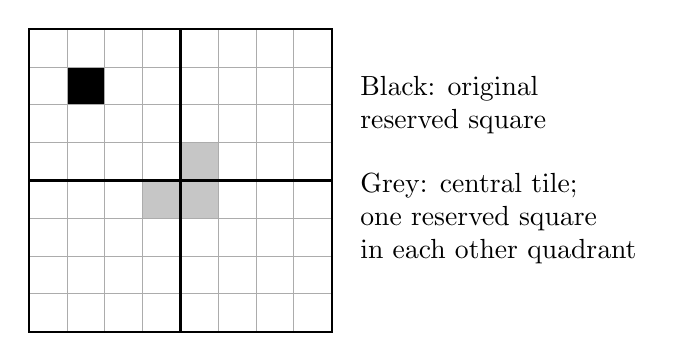
\begin{tikzpicture}[scale=0.48]
\fill[black] (1,6) rectangle (2,7);
\fill[gray!45] (4,4) rectangle (5,5);
\fill[gray!45] (3,3) rectangle (5,4);
\draw[step=1,gray!65,thin] (0,0) grid (8,8);
\draw[thick] (0,0) rectangle (8,8);
\draw[very thick] (4,0)--(4,8) (0,4)--(8,4);
\node[right,align=left] at (8.5,6) {Black: original\\reserved square};
\node[right,align=left] at (8.5,3) {Grey: central tile;\\one reserved square\\in each other quadrant};
\end{tikzpicture}
\caption{One placement creates four smaller instances of the same task.}
\end{figure}

\paragraph{Correctness by induction on $n$.}
For $n=0$, the only square is reserved, so no tile is needed. Assume, for
some integer $k\geq0$, that the procedure correctly completes every
$2^k\times2^k$ region satisfying its precondition, without changing any
reserved square or any square outside the region. Consider a region of
side $2^{k+1}$. Its three chosen central squares are empty and form an L,
so the placement is legal. Each quadrant now has exactly one reserved
square, and its other squares remain empty. The induction hypothesis
applies to each call. The quadrants are disjoint, and each call leaves the
others alone. Together the four completed tilings and the central tile
cover exactly the required squares, with no overlap. This proves the step.
The quadrant loop has bound function $4-j$, decreasing by one per
completed call. Each call finishes by induction on $n$: its subcalls
have parameter $n-1$, and at $n=0$ there are none. Thus the loop bound
and the decreasing recursive parameter together establish termination.

If $T(n)$ counts tiles placed, then
\[
T(0)=0,\qquad T(n)=4T(n-1)+1\quad(n\geq1),
\qquad T(n)=\frac{4^n-1}{3}.
\]
The last equality follows by unfolding the recurrence or by counting squares.
With constant work per call apart from its subcalls, the running time is
proportional to the board's area $4^n$. It is exponential in $n$, but linear
in the number of squares to be covered. Here the size parameter matters:
the produced tiling itself contains that many pieces of information.

\subsection{The Tower of Hanoi: a computation that produces actions}

Three pegs hold $n$ disks of different sizes. Initially all disks are on
one peg, with smaller disks above larger ones. Move the tower to another
peg, moving only one top disk at a time and never placing a larger disk
on a smaller one. The third peg is available as a spare.

\begin{figure}[ht]
\centering
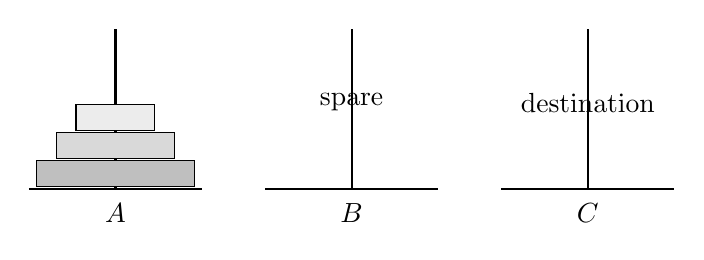
\begin{tikzpicture}[x=1cm,y=0.55cm]
\foreach \x/\name in {0/A,3/B,6/C}{
\draw[thick] (\x-1.1,0)--(\x+1.1,0);
\draw[thick] (\x,0)--(\x,3.7);
\node at (\x,-0.55) {$\name$};}
\filldraw[fill=gray!50] (-1,0.05) rectangle (1,0.65);
\filldraw[fill=gray!30] (-0.75,0.7) rectangle (0.75,1.3);
\filldraw[fill=gray!15] (-0.5,1.35) rectangle (0.5,1.95);
\node at (3,2) {spare};\node at (6,2) {destination};
\end{tikzpicture}
\caption{Three disks initially on $A$. Move the whole tower to $C$.}
\end{figure}

To uncover the largest disk, first move all smaller disks to the spare
peg. Then move the largest disk to the destination. Finally move the
smaller tower onto it. The proof suggests the procedure directly.

The promised result is that the specified tower moves from $A$ to $C$
in legal order, using only legal moves, and all larger disks remain where
they were. Allowing larger disks underneath the moving tower is important:
that is the situation faced by the recursive calls.

Throughout these actions the disks must remain distributed among the
three pegs without loss or duplication, each peg must have smaller disks
above larger ones, and all disks outside the specified tower must remain
in place. These are the properties to preserve. Since this procedure is
recursive rather than a loop, its main correctness argument will use the
inductive specification of each call.

\begin{algorithm}[H]
\begin{algorithmic}[1]
\Procedure{Hanoi}{$n,A,B,C$}
\Statex \texttt{\# PRE:} $n\in\mathbb N$. The $n$ disks form a top tower on $A$; the pegs are distinct.
Any other disks on the three pegs are larger than these $n$ disks.
\Statex \texttt{\# INV (safety):} no disks lost or duplicated; each peg remains ordered;
\Statex \texttt{\#} all disks outside this tower remain in place.
\If{$n>0$}
\State Call \Call{Hanoi}{$n-1,A,C,B$}.
\Statex \texttt{\# ASSERT:} the smaller tower is on $B$; the largest disk is exposed on $A$.
\State Move the top disk from $A$ to $C$.
\State Call \Call{Hanoi}{$n-1,B,A,C$}.
\EndIf
\Statex \texttt{\# POST:} the specified tower is on $C$ in order, all moves were legal,
\Statex \texttt{\#} and every other disk is unchanged.
\EndProcedure
\end{algorithmic}
\caption{Move $n$ disks from the first named peg to the last, using the middle peg as spare.}
\end{algorithm}

\paragraph{Correctness by induction on $n$.}
For $n=0$, doing nothing meets the specification. Suppose for some integer
$k\geq0$ that every call moving $k$ disks satisfies the specification.
In a call moving $k+1$ disks, the first recursive call legally moves the
$k$ smaller disks from $A$ to $B$, leaving the largest disk exposed.
The top of $C$ is empty or larger than that disk, so the single move from
$A$ to $C$ is legal. The second recursive call legally moves the smaller
tower from $B$ to $C$, on top of the disk just moved. Both calls preserve
all larger disks. This proves the step. The call parameter decreases to
zero, proving termination.

For two disks, the actions are $A\to B$, $A\to C$, $B\to C$.
For three disks, they are
\[
A\to C,\ A\to B,\ C\to B,\ A\to C,\ B\to A,\ B\to C,\ A\to C.
\]
Each arrow means ``move the top disk'', not ``move the entire tower''.
The output is an ordered sequence of actions. Changing their order can
make a move illegal, even if the same peg names occur.

If $H(n)$ counts moves, then
\[
H(0)=0,\qquad H(n)=2H(n-1)+1\quad(n\geq1).
\]
Adding one on both sides and unfolding gives $H(n)+1=2^n$, so
$H(n)=2^n-1$. This exponential growth is unavoidable for three pegs.
Before the first move of the largest disk, all smaller disks must have
been transferred to a single other peg. After the last move of the largest
disk onto its destination, all smaller disks again form a tower on another
peg and must be transferred onto it. These are two separate transfers of
$n-1$ disks, with at least one move of the largest disk between them.
Thus, if $M(n)$ is the minimum number of moves,
$M(n)\geq2M(n-1)+1$. Induction on $n$, with base $M(0)=0$ and step
$M(k+1)\geq2(2^k-1)+1=2^{k+1}-1$ for every integer $k\geq0$, gives the
lower bound. Our procedure attains it.

At one move per second, $64$ disks require about $585$ billion years.
A short recursive description can specify a very long computation.
\footnote{\'Edouard Lucas published the puzzle in 1883 under the name
N.~Claus de Siam, an anagram of Lucas d'Amiens. Its accompanying temple
story is part of the puzzle's presentation, not evidence of an ancient
algorithm. See the \href{https://mathshistory.st-andrews.ac.uk/Extras/Hanoi/}{MacTutor historical account}.}

\section{What the two models share}

For a tail-recursive procedure, the arguments describing the current state
become stored variables; the stopping test becomes a loop condition;
and the recursive transition becomes the loop body. Its invariant carries
over. Separate assignments must implement the intended transition correctly,
which may require temporary storage.

For general recursion, unfinished calls also form part of the state. Hanoi
must remember to move the largest disk and make the second call after its
first call finishes. A stack can record these pending tasks. We can in
principle replace recursive calls by a loop processing such a stack, but
this does not remove the pending work or its storage requirements.
Recursion and iteration remain different ways of organising computation
within an imperative description.

The functional viewpoint emphasises how an answer is built from answers
to smaller problems. The imperative viewpoint emphasises how instructions
change a stored state. Neither confines us to numerical answers: a tiling,
a reversed list, or a sequence of moves can be represented as finite data.
The numerical model of Chapter~\ref{chap:algorithms} can encode such data; here
we describe it in the form most natural for the task.

The thread connecting all these examples is the proof. An induction tells
us how to divide a recursive task. An invariant tells us how to change a
state without losing the relationship that leads to the answer. In both
cases, reasoning is part of constructing the procedure.

\section*{Problems}
For each loop you design, first state its postcondition, generalise it to
an invariant, and then derive the commands. Give a nonnegative integer
bound function and show that it strictly decreases on every iteration.
\begin{enumerate}
\setlength{\itemsep}{1pt}\setlength{\parsep}{0pt}
\item Start with $x=3,y=7$. Trace $x\leftarrow x+y$ followed by
$y\leftarrow x-y$. Add one assignment that exchanges the original values.
Explain why a temporary location is often easier to reason about.
\item Translate $(u,v)\mapsto(v,u+v)$ into sequential assignments.
Give a failing translation and explain which old value it loses.
\item Trace Factorial for $n=0$ and $n=5$. At which point inside the body
can its invariant fail? Show that it is restored before the next test.
\item Design an increasing-counter factorial loop with invariant
$p=k!$ and $0\leq k\leq n$. Give initialisation, preservation, exit, and
termination arguments. Compare its update order with Factorial.
\item Translate repeated-addition multiplication into a loop. Use the
invariant $p+ak=ab$ from Section~\ref{sec:alg-iterative-examples}, with
fixed inputs $a,b\geq0$. Count additions.
\item Construct an imperative power procedure from $p x^k=X^N$, where
$X,N$ are fixed inputs. Compare Sections~\ref{sec:alg-fast-power}
and~\ref{sec:alg-iterative-examples}. Use even and odd cases to halve $k$ on each
repetition. Specify assignment order and prove correctness.
\item Trace Sum for $f(i)=i^2$, $a=2$, $b=5$. Explain why advancing $k$
before adding $f(k)$ changes the terms summed. Handle $a>b$.
\item Trace Divide for $(23,4)$. Prove that its repetition count is the
quotient. Explain why $b>0$ is necessary for termination.
\item Replace Euclid's body by $u\leftarrow v$ followed by
$v\leftarrow\operatorname{mod}(u,v)$. Find a counterexample and explain
the failure in terms of storage.
\item Give a loop and a true invariant for which the loop never ends.
Explain which part of a correctness proof is missing.
\item Trace Reverse on lists of lengths $0,1,2$, and $6$. Prove that no
entry outside the list is accessed. Count the temporary locations needed.
\item Design a procedure that finds a largest entry of a nonempty list.
Use an invariant describing the largest entry in the processed prefix.
State what happens when the largest value occurs more than once.
\item Draw every tile placed by Tile on a $4\times4$ board with one
corner missing. Repeat with an interior square missing. Label the order
of placements, following the stated quadrant order.
\item Why must Tile permit a reserved square that is already occupied?
Explain why ``one square is physically missing'' is not a suitable
specification for every recursive call.
\item Prove $T(n)=(4^n-1)/3$ from its recurrence by induction on $n$,
explicitly quantifying the induction hypothesis. Relate this to area.
\item Trace Hanoi for three disks, recording the peg state after each
move. Check legality as well as the final destination.
\item Prove the lower bound for Hanoi by induction on the number of disks.
Which step relies on having exactly three pegs and fails with a fourth?
\item Describe a stack of pending Hanoi tasks that a loop could process.
In what order must tasks be placed on a last-in, first-out stack to reproduce
the recursive procedure? Distinguish the task stack from the pegs.
\item For Exchange, Sum, Tile, and Hanoi, state the input, output or changed
state, and permitted actions. Explain how the non-numerical data could,
in principle, be encoded by natural numbers.
\item Trace SequentialSearch on a list containing several copies of its target.
Prove that it returns the first occurrence. Give its best and worst cases.
\item Trace BinarySearch for an absent target smaller than every entry,
larger than every entry, and between two consecutive entries. Include the
empty list and the one-entry list.
\item Modify BinarySearch to return the first occurrence of its target.
State a new invariant that records a possible answer as the interval shrinks.
\item Find an unsorted list on which BinarySearch incorrectly reports
absence. Identify precisely which preservation argument fails.
\item In Stage 1 of insertion sort, why is a sorted prefix alone an
incomplete invariant? Explain the roles of multiplicities and unchanged entries.
\item Starting from the assertion $Q$, justify every clause of the inner
invariant. Give an example where the entire stored list is temporarily
not a rearrangement of its original contents.
\item Give a nonnegative real-valued function that strictly decreases
in an infinite loop. Explain why our definition requires integer values.
\item Give bound functions for both searches, including successful
iterations. Why does the number of uninspected entries alone fail to
strictly decrease on a successful iteration?
\item Trace every assignment while inserting $1$ into the sorted prefix
$[2,4,5]$. Mark the logical hole and the saved value after each shift.
\item Why does replacing $L[j-1]>x$ by $L[j-1]\geq x$ in InsertionSort
still sort the values but change the order in which equal entries can finish?
Use labelled cards such as $2_a$ and $2_b$ to illustrate.
\item Prove that insertion sort makes exactly $m(m-1)/2$ shifts on
$m$ distinct entries presented in decreasing order. State the induction
parameter and quantify the induction hypothesis.
\item Suppose an unchanging list of length $m$ will be searched $q$ times.
Compare $q$ linear searches with insertion sort followed by $q$ binary
searches, using the bounds in this chapter. Explain why these bounds alone
do not determine an exact practical crossover point.
\end{enumerate}
